% -*- root: ../main.tex -*-

\documentclass[../main.tex]{subfiles}
\begin{document}

\chapter{Reduzierte-Basis-Methode} % (fold)
\label{chapter:rbm}

Aufbauend auf das Petrov"=Galerkin"=Verfahren des vorherigen Kapitels führen wir nun die Reduzierte"=Basis"=Methode (kurz RB"=Methode) ein.
Zunächst folgen einige theoretische Grundlagen und Ausführungen zur numerischen Umsetzung dieser Methode, bevor wir mit einigen beispielhaften Anwendungen auf die betrachtete Problemstellung abschließen.

\section{Grundlagen} % (fold)
\label{sub:grb:rb:grundlagen}

Wir beginnen mit einer kurzen Motivation und orientieren uns in diesem Abschnitt an den Arbeiten von \textcite{Rozza2008} sowie \textcite{Patera:2007un}, welche einen weit tieferen Einblick bieten.
Bei der Reduzierte"=Basis"=Methode handelt es sich um ein relativ junges Verfahren, welches vor allem in den letzten zehn Jahren viel Aufmerksamkeit und Weiterentwicklung erfahren hat.

Zunächst wollen wir erneut geeignete Rahmenbedingungen in Form eines abstrakten Variationsproblems schaffen.
Seien dazu zwei Hilberträume $\mathcal X$ und $\mathcal Y$ und eine abgeschlossene, konvexe Parametermenge $\mathcal P \subset \mathbb{R}^{p}$ für ein $p \in \mathbb{N}$ gegeben.
Weiter seien $b \colon \mathcal X \times \mathcal Y \times \mathcal P \to \mathbb{R}$ eine parametrische stetige Bilinearform und $f \colon \mathcal Y \to \mathbb{R}$ ein stetiges lineares Funktional.
Wir betrachten das abstrakte parametrische Variationsproblem:
\begin{equation}
\label{eq:abstraktes_parametrische_vp}
    \text{Sei } \bm \sigma \in \mathcal P, \text{ finde } u(\bm \sigma) \in \mathcal X \text{ mit} \quad b(u(\bm \sigma), v; \bm \sigma) = f(v) \quad \fa v \in \mathcal Y.
\end{equation}

Reduzierte"=Basis"=Methoden bieten sich dann an, wenn das Variationsproblem für einen gegebenen Parameter in Echtzeit oder immer wieder für viele verschiedene Parameter gelöst werden muss.
Um dies mit zufriedenstellender Genauigkeit effizient bewerkstelligen zu können, konzentriert man sich auf die Lösungsmenge
\begin{equation}
\label{eq:stetige_loesungsmenge}
    \mathcal M := \Set{u(\bm \sigma) \in \mathcal X \given \bm \sigma \in \mathcal P}.
\end{equation}
Erfüllt die Bilinearform aus \cref{eq:abstraktes_parametrische_vp} gewisse Regularitätseigenschaften bezüglich des Parameters, dann bildet $\mathcal M$ oftmals eine Mannigfaltigkeit mit vergleichsweise niedriger Dimension.

Um diese Tatsache ausnutzen zu können, müssen wir $\mathcal M$ zunächst durch ein diskretes Analogon ersetzen.
Dazu werden bei den klassischen Reduzierte"=Basis"=Methoden Galerkin"=Verfahren verwendet, weswegen wir an dieser Stelle das Petrov"=Galerkin"=Verfahren des vorherigen Kapitels nutzen um eine abstrakte Diskretisierung durchzuführen.
Seien $\mathcal X_{\mathcal N} \subset \mathcal N$ und $\mathcal Y_{\mathcal N} \subset \mathcal Y$ Unterräume der Dimension $\mathcal N \in \mathbb{N}$.
Weiter nehmen wir an, dass diese Diskretisierung für alle $\bm \sigma \in \mathcal P$ zu einem korrekt gestellten Variationsproblem führt, welches gegeben sei durch:
\begin{equation}
\label{eq:diskretes_abstraktes_parametrisches_vp}
    \text{Sei } \bm \sigma \in \mathcal P, \text{ finde } u_{\mathcal N}(\bm \sigma) \in \mathcal X_{\mathcal N} \text{ mit} \quad b(u_{\mathcal N}(\bm \sigma), v; \bm \sigma) = f(v) \quad \fa v \in \mathcal Y_{\mathcal N}.
\end{equation}
Da die RB"=Methode maßgeblich auf diese Petrov"=Galerkin"=Diskretisierung und nicht das eigentliche Variationsproblem \cref{eq:abstraktes_parametrische_vp} aufbaut, werden wir \cref{eq:diskretes_abstraktes_parametrisches_vp} mit dem Präfix \emph{Truth} kenntlich machen.
Die Truth"=Lösungsmenge sei nun definiert als
\begin{equation}
\label{eq:truth_loesungsmenge}
    \mathcal M_{\mathcal N} := \Set{u_{\mathcal N}(\bm \sigma) \in \mathcal X_{\mathcal N} \given \bm \sigma \in \mathcal P}.
\end{equation}
Dies erlaubt die Konstruktion eines niedrigdimensionalen Unterraums $\mathcal X_{N} \subset \mathcal M_{\mathcal N} \subset \mathcal X_{\mathcal N}$, welcher als Ansatzraum eines weiteren Galerkin"=Verfahrens dienen wird.
Dies ist die Grundidee der RB"=Methoden, die in \cref{figure:rbm_loesungsmenge} noch einmal skizzenhaft veranschaulicht wird.

\begin{figure}[tb]
    \centering
    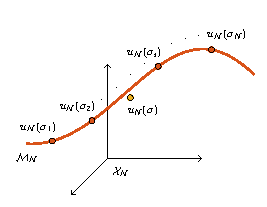
\includegraphics[width=0.5\textwidth]{figures/rb.pdf}
    \caption[%
    Skizze zur Motivation der Reduzierte-Basis-Methode.
    ]{
        Skizze der Funktionsweise der Reduzierte"=Basis"=Methode im Falle eines eindimensionalen Parameters $\sigma$.
        Die Reduzierte"=Basis"=Lösungen $u_{N}(\sigma)$ ergeben sich als Linearkombinationen der Truth"=Lösungen $u_{\mathcal N}(\sigma_{i})$ für gewisse $\sigma_{i} \in \mathcal P$.
        }
    \label{figure:rbm_loesungsmenge}
\end{figure}

Die Konstruktion des niedrigdimensionalen Ansatzraumes $\mathcal X_{N}$ erfolgt unter dem Aspekt, den durch das zweite Galerkin"=Verfahren zusätzlich eingeführten Fehler für alle Parameter des Parameterraums $\mathcal P$ zu minimieren, was in einem hohen Rechenaufwand resultiert.
Dies motiviert die bei RB"=Methoden übliche Zerlegung in ein zwei Stufen.
Die erste Stufe, die sogenannte \emph{Offline-Phase}, dient dazu den Ansatzraum $\mathcal X_{N}$ unter dem genannten Gesichtspunkt zu konstruieren und muss nur einmal ausgeführt werden.
In der zweiten Stufe, der \emph{Online-Phase}, kann dieses niedrigdimensionale System verwendet werden, um Lösungen für gegebene Parameter auszuwerten und eine garantierte Fehlerschranke zu berechnen.
Da im Allgemeinen $N \ll \mathcal N$ gilt, wird hierbei als weiteres Ziel die Unabhängigkeit der Berechnungen in der Online-Phase von der Dimension $\mathcal N$ verfolgt.

Weiter führt diese Zerlegung zu einem wichtigen Kriterium für respektive gegen die Anwendung der RB"=Methode, da der benötigte Aufwand für die Offline-Phase meist erst ab einer hohen Anzahl an zu bestimmenden Lösungen in der Online-Phase amortisiert wird.

Wir widmen uns nun den formalen Grundlagen der RB"=Methode und beginnen mit einer grundlegenden Definition.

\begin{Definition}
\label{definition:rb_variationsproblem}
    Es seien $N \in \mathbb{N}$ und $\mathcal S_{N} := \Set{ \bm \sigma_{n} \given n = 1, \dots, N } \subset \mathcal P$ die sogenannte \emph{Sample-Menge}.
    Wir bezeichnen die Truth-Lösungen $u_{\mathcal N}(\bm \sigma_{n})$ als \emph{Snapshots} und definieren den \emph{RB"=Ansatzraum} $\mathcal X_{N}$ als
    \begin{equation}\label{eq:def_rb_ansatzraum}
        \mathcal X_{N} := \spn \Set{ u_{\mathcal N}(\bm \sigma_{n}) \given n = 1, \dots, N} = \spn \Set{ \xi_{n} \given n = 1, \dots, N},
    \end{equation}
    wobei $\Xi_{N} := \Set{ \xi_{n} \given n = 1, \dots, N}$ eine geeignete Orthonormalbasis ist, sowie einen $N$-dimensionalen \emph{RB"=Testraum}  $\mathcal Y_{N} \subset \mathcal Y_{\mathcal N}$.
    Als \emph{RB"=Variationsproblem} von \cref{eq:diskretes_abstraktes_parametrisches_vp} bezeichnen wir das  Variationsproblem:
    \begin{equation}
    \label{eq:rb_abstraktes_parametriches_vp}
        \text{Sei } \bm \sigma \in \mathcal P, \text{ finde } u_{N}(\bm \sigma) \in \mathcal X_{N} \text{ mit} \quad b(u_{N}(\bm \sigma), v; \bm \sigma) = f(v) \quad \fa v \in \mathcal Y_{N}.
    \end{equation}
    Fernen nennen wir $u_{N}(\bm \sigma)$ \emph{Reduzierte"=Basis"=Lösung}.
\end{Definition}

RB-Ansatzräume der Art \cref{eq:def_rb_ansatzraum} werden in der Literatur zu RB-Methoden auch als \emph{Lagrangeräume} bezeichnet, um sie damit von komplexeren Räumen, wie beispielsweise \emph{Taylor-} und \emph{Hermiteräumen} abzugrenzen.
Bei diesen werden neben den Truth-Lösungen auch deren partielle Ableitungen bezüglich der Parameter berücksichtigt.
Eine Übersicht darüber findet sich in \cite[Chapter 3]{Patera:2007un}.

Wie zuvor bei den Petrov"=Galerkin"=Verfahren muss auch bei \cref{eq:rb_abstraktes_parametriches_vp} sichergestellt werden, dass es sich dabei um ein korrekt gestelltes Problem handelt.
Wir werden später sehen, dass diese Eigenschaft bei geschickter Wahl des Testraumes $\mathcal Y_{N}$ vom Truth"=Variationsproblem vererbt wird, und nehmen deswegen an dieser Stelle an, dass dies stets erfüllt ist.

Da es sich bei der RB"=Diskretisierung ebenfalls um ein Galerkin"=Verfahren handelt, erhalten wir Analoga der Aussagen \cref{satz:galerkin_stabilitaet} sowie \cref{satz:lemma_von_cea}, welche hier nicht wiederholt werden, wobei die Truth-Räume $\mathcal X_{\mathcal N}$ und $\mathcal Y_{\mathcal N}$ die Rolle der Hilberträume $\mathcal X$ und $\mathcal Y$ einnehmen.

Weiter soll an dieser Stelle angemerkt werden, warum wir eine Galerkin"=Diskretisierung \cref{eq:diskretes_abstraktes_parametrisches_vp} als Grundlage und nicht das eigentliche Variationsproblem \cref{eq:abstraktes_parametrische_vp} verwenden.
Neben dem offensichtlichen Grund, der Berechenbarkeit der Lösung, ist die zugrundeliegende Prämisse die Folgende:
Nach \cref{satz:lemma_von_cea} kann mit der Petrov"=Galerkin"=Lösung $u_{\mathcal N}(\bm \sigma)$ die exakte Lösung $u(\bm \sigma)$ unter gewissen Annahmen beliebig gut approximiert werden.
Betrachten wir weiter die einfache Abschätzung
\begin{equation}
    \norm{u(\bm \sigma) - u_{N}(\bm \sigma)}_{\mathcal X} \leq \norm{u(\bm \sigma) - u_{\mathcal N}(\bm \sigma)}_{\mathcal X} + \norm{u_{\mathcal N}(\bm \sigma) - u_{N}(\bm \sigma)}_{\mathcal X},
\end{equation}
dann entspricht dies gerade der Tatsache, das der erste Summand beliebig klein gehalten werden kann.
Dies erlaubt uns lediglich den Fehler zwischen Truth- und RB"=Lösung zu berücksichtigen und führt weiter zu folgender Definition.

\begin{Definition}\label{definition:rbm_fehler_und_residuum}
    Als \emph{Fehler} $e_{N}(\bm \sigma) \in \mathcal X_{\mathcal N}$ bezeichnen wir $e_{N}(\bm \sigma) := u_{\mathcal N}(\bm \sigma) - u_{N}(\bm \sigma)$.
    Weiter definieren wir das \emph{Residuum} $r_{N}(\blank; \bm \sigma) \colon \mathcal Y_{\mathcal N} \to \mathbb{R}$ als
    \begin{equation}\label{eq:variationsproblem_residuum}
        r_{N}(v; \bm \sigma) := b(e_{N}(\bm \sigma), v; \bm \sigma), \quad v \in \mathcal Y_{\mathcal N}.
    \end{equation}
\end{Definition}

\begin{Lemma}\label{lemma:rbm_residuum_ist_funktional}
    Das Residuum $r_{N}(\blank; \bm \sigma)$ ist für alle $\bm \sigma \in \mathcal P$ ein stetiges lineares Funktional, kurz also $r_{N}(\blank; \bm \sigma) \in \mathcal Y_{\mathcal N}'$.

    \begin{Beweis}
        Sowohl Linearität als auch Stetigkeit sind direkt ersichtlich, denn nach Definition erhalten wir
        \begin{equation}\label{eq:residuum_durch_funktional_und_bilinearform}
            \begin{aligned}
            r_{N}(v; \bm \sigma)
            &= b(e_{N}(\bm \sigma), v; \bm \sigma)
            = b(u_{\mathcal N}(\bm \sigma), v; \bm \sigma) - b(u_{N}(\bm \sigma), v; \bm \sigma)
            \\&= f(v) - b(u_{N}(\bm \sigma), v; \bm \sigma)
            \end{aligned}
        \end{equation}
        und diese Eigenschaften damit von $f$ und $b$.
    \end{Beweis}
\end{Lemma}

Das Residuum kann nun verwendet werden, um eines der wichtigsten Konstrukte der RB-Methoden zu definieren.

\begin{Lemma}\label{lemma:rbm_fehler_schranke}
    Sei $\beta_{\mathrm{LB}}(\bm \sigma) > 0$ eine untere Schranke für $\beta_{\mathcal N}(\bm \sigma)$.
    Dann gilt
    \begin{equation}
        \norm{u_{\mathcal N}(\bm \sigma) - u_{N}(\bm \sigma)}_{\mathcal X} \leq \Delta_{N}(\bm \sigma) := \frac{\norm{r_{N}(\blank; \bm \sigma)}_{\mathcal Y_{\mathcal N}'}}{\beta_{\mathrm{LB}}(\bm \sigma)},
    \end{equation}
    wobei wir $\Delta_{N}(\bm \sigma)$ als \emph{a posteriori-Fehlerschätzer} bezeichnen.

    \begin{Beweis}
        Wir können \cref{eq:variationsproblem_residuum} als Variationsproblem \cref{eq:diskretes_abstraktes_parametrisches_vp} auffassen, welches unter den getroffenen Annahmen die eindeutige Lösung $e_{N}(\bm \sigma)$ besitzt.
        Die Abschätzung folgt nun aus \cref{satz:galerkin_stabilitaet}.
    \end{Beweis}
\end{Lemma}

Dieser a posteriori-Fehlerschätzer bildet das Herzstück der RB"=Methode, da mit ihm in der Offline-Phase eine möglichst optimale Wahl der Parameter-Samples erreicht werden kann, während er in der Online-Phase zur Berechnung einer garantierten Fehlerschranke zwischen Truth- und RB-Lösung verwendet wird.
Dazu setzt man weiter woraus, dass die untere Schranke $\beta_{\mathrm{LB}}(\bm \sigma)$ berechenbar ist.
Wir werden bei der nachfolgenden numerischen Umsetzung darauf eingehen, wie dies bewerkstelligt werden kann.

Bevor wir uns dieser widmen, wollen wir an dieser Stelle noch ein Maß für die Güte des Fehlerschätzers einführen.

\begin{Lemma}
\label{lemma:effektivitaet}
    Die \emph{Effektivität} $\eta_{N}(\bm \sigma)$ des a posteriori"=Fehlerschätzers ist beschränkt durch
    \begin{equation}
        1 \leq \eta_{N}(\bm \sigma) := \frac{\Delta_{N}(\bm \sigma)}{\norm{u_{\mathcal N}(\bm \sigma) - u_{N}(\bm \sigma)}_{\mathcal X}} \leq \frac{\gamma_{\mathcal N}(\bm \sigma)}{\beta_{\mathrm{LB}}(\bm \sigma)},
    \end{equation}
    wobei $\gamma_{\mathcal N}(\bm \sigma)$ die Stetigkeitskonstante der Bilinearform $\restr{b(\blank, \blank; \bm \sigma)}{\mathcal X_{\mathcal N} \times \mathcal Y_{\mathcal N}}$ sei.

    \begin{Beweis}
        Die Abschätzung nach unten ergibt sich direkt aus \cref{lemma:rbm_fehler_schranke}.
        Sei nun $\bm \sigma \in \mathcal P$ beliebig.
        Eine Anwendung des Rieszschen Darstellungssatz liefert für $r_{N}(\blank; \bm \sigma)$ ein $\hat{e}_{N} \in \mathcal Y_{\mathcal N}$ mit $r_{N}(v; \bm \sigma) = \skp{\hat{e}_{N}}{v}{\mathcal Y}$ für alle $v \in \mathcal Y_{\mathcal N}$ und $\norm{r_{N}(\blank; \bm \sigma)}_{\mathcal Y_{\mathcal N}'} = \norm{\hat{e}_{N}}_{\mathcal Y}$.
        Mit der Stetigkeit der Bilinearform erhalten wir damit die Abschätzung
        \begin{equation}
            \norm{\hat{e}_{N}}_{\mathcal Y}^{2}
            = \skp{\hat{e}_{N}}{\hat{e}_{N}}{\mathcal Y}
            = r_{N}(\hat{e}_{N}; \bm \sigma)
            = b(e_{N}(\bm \sigma), \hat{e}_{N}; \bm \sigma)
            \leq \gamma_{\mathcal N}(\bm \sigma) \norm{e_{N}(\bm \sigma)}_{\mathcal X} \norm{\hat{e}_{N}}_{\mathcal Y},
        \end{equation}
        oder kurz
        \begin{equation}
            \norm{\hat{e}_{N}}_{\mathcal Y} \leq \gamma_{\mathcal N}(\bm \sigma) \norm{e_{N}(\bm \sigma)}_{\mathcal X}.
        \end{equation}
        Zusammen mit der Definition des a posteriori"=Fehlerschätzers $\Delta_{N}(\bm \sigma)$ liefert dies nun
        \begin{equation}
            \eta_{N}(\bm \sigma)
            = \frac{\Delta_{N}(\bm \sigma)}{\norm{u_{\mathcal N}(\bm \sigma) - u_{N}(\bm \sigma)}_{\mathcal X}}
            \leq \frac{\gamma_{\mathcal N}(\bm \sigma) \norm{e_{N}(\bm \sigma)}_{\mathcal X}}{\beta_{\mathrm{LB}}(\bm \sigma)\norm{u_{\mathcal N}(\bm \sigma) - u_{N}(\bm \sigma)}_{\mathcal X}}
            = \frac{\gamma_{\mathcal N}(\bm \sigma)}{\beta_{\mathrm{LB}}(\bm \sigma)}.
        \end{equation}
    \end{Beweis}
\end{Lemma}

Dieses Ergebnis ist wichtig, denn es garantiert, dass der a posteriori-Fehlerschätzer weder zu pessimistisch noch zu optimistisch ist.
Insbesondere garantiert es, dass der tatsächliche Fehler durch den a posteriori-Fehlerschätzer stets korrekt nach oben abgeschätzt wird.

% TODO: noch etwas zur Konvergenz sagen?

\section{Numerische Umsetzung} % (fold)
\label{section:cha5_rbm:numerische_umsetzung}

Wir richten unsere Aufmerksamkeit nun auf die numerische Umsetzung der RB"=Methode und orientieren uns dabei weiterhin an \cite{Rozza2008,Patera:2007un}.
Zunächst abstrahieren wir die aus \cref{lemma:bilinearform_affin_parametrisch} bekannte affine Abhängigkeit der parametrischen Bilinearform des Variationsproblems \cref{eq:abstraktes_parametrische_vp}.

\begin{Definition}
\label{definition:parametrisch_affine_bf_fuer_rbm}
    Wir nennen eine parametrische Bilinearform $b \colon \mathcal X \times \mathcal Y \times \mathcal P \to \mathbb{R}$ \emph{parametrisch affin}, wenn sie die Form
    \begin{equation}\label{eq:bilinearform_parametrisch_affin}
        b(u, v; \bm \sigma) = \sum_{q = 1}^{Q_{b}} \theta_{q}^{b}(\bm \sigma) b_{q}(u, v), \quad \text{für } u \in \mathcal X,~v \in \mathcal Y,~\bm \sigma \in \mathcal P,
    \end{equation}
    hat, wobei für $q = 1, \dots, Q_{b}$ durch $\theta_{q}^{b} \colon \mathcal P \to \mathbb{R}$ Funktionen und durch $b_{q} \colon \mathcal X \times \mathcal Y \to \mathbb{R}$ parameterunabhängige Bilinearformen gegeben seien.
\end{Definition}

Für dieses Kapitel nehmen wir ferner an, dass die Funktionen $\theta_{q}^{b}$ effizient ausgewertet werden können.
Weiter vereinfachen wir an dieser Stelle die Notation aus \cref{section:galerkin_numerische_umsetzung}.
Die endlichdimensionalen Räume $\mathcal X_{\mathcal N}$ und $\mathcal Y_{\mathcal N}$ der Truth"=Diskretisierung fassen wir als Span entsprechender Basen auf und schreiben
\begin{equation}
    \mathcal X_{\mathcal N} = \spn \Set{ \phi_{i} }_{ i = 1, \dots, \mathcal N },
    \qquad
    \mathcal Y_{\mathcal N} = \spn \Set{ \psi_{j} }_{ j = 1, \dots, \mathcal N }.
\end{equation}
Analog verfahren wir für die $N$-dimensionalen RB"=Räume $\mathcal X_{N}$ und $\mathcal Y_{N}$ mit der Notation
\begin{equation}
    \mathcal X_{N} = \spn \Set{ \xi_{n} }_{ n = 1, \dots, N},
    \qquad
    \mathcal Y_{N} = \spn \Set{ \eta_{m} }_{ m = 1, \dots, N}.
\end{equation}
Die bei der Petrov"=Galerkin"=Diskretisierung hergeleiteten Strukturen $\mat{X}, \mat{Y}, \mat{B}_q \in \mathbb{R}^{\mathcal N \times \mathcal N}$ mit $q = 1, \dots, Q_b$ und $\vec{f} \in \mathbb{R}^{\mathcal N}$ lassen sich damit kurz schreiben als
\begin{equation}
    \begin{aligned}
        \mat{X} &= \left[ \skp{\phi_{i}}{\phi_{j}}{\mathcal X} \right]_{i,j = 1, \dots, \mathcal N},
        &\qquad
        \mat{Y} &= \left[ \skp{\psi_{i}}{\psi_{j}}{\mathcal Y} \right]_{i,j = 1, \dots, \mathcal N},
        \\
        \vec{f} &= \left[ f(\psi_{j}) \right]_{j = 1, \dots, \mathcal N},
        &\qquad
        \mat{B}_{q} &= \left[ b_{q}(\phi_{i}, \psi_{j}) \right]_{j,i = 1, \dots, \mathcal N}.
    \end{aligned}
\end{equation}
Nach diesen Vorbemerkungen geben wir nun als ersten Schritt eine Möglichkeit zur Bestimmung der Reduzierte"=Basis"=Äquivalente dieser Strukturen an.

\begin{Definition}\label{definition:rb_ansatz_und_testfunktionen}
    Als \emph{Reduzierte"=Basis"=Ansatzfunktion} $u_{N} \in \mathcal X_{N}$ respektive \emph{Testfunktion} $v_{N} \in \mathcal Y_{N}$ bezeichnen wir die Linearkombinationen
    \begin{equation}
        u_{N} := \sum_{n = 1}^{N} u_{n, N} \xi_{n},
        \qquad
        v_{N} := \sum_{m = 1}^{N} v_{m, N} \eta_{m}
    \end{equation}
    mit den Koeffizientenvektoren $\vec{u}_{N} := [u_{n, N}]_{n = 1, \dots, N}, \vec{v}_{N} := [v_{m,N}]_{m = 1, \dots, N} \in \mathbb{R}^{N}$.
\end{Definition}

Nach Konstruktion können die Basisfunktionen $\Set{ \xi_{n} }_{ n = 1, \dots, N}$ und $\Set{ \eta_{m} }_{ m = 1, \dots, N}$ jeweils als Linearkombination von $\Set{ \phi_{i} }_{ i = 1, \dots, \mathcal N}$ beziehungsweise $\Set{ \psi_{j} }_{ j = 1, \dots, \mathcal N}$ geschrieben werden.
Bezeichnen wir nun für $n,m = 1, \dots, N$ die entsprechenden Koeffizientenvektoren mit $\bm \xi_{n}, \bm \eta_{m} \in \mathbb{R}^{\mathcal N}$, dann können wir damit weiter die Matrizen
\begin{equation}
  \mat{\Xi} := [\bm \xi_{n}]_{n = 1, \dots, N} \in \mathbb{R}^{\mathcal N \times N},
  \qquad
  \mat{H}   := [\bm \eta_{m}]_{m = 1, \dots, N} \in \mathbb{R}^{\mathcal N \times N}
\end{equation}
definieren.
Diese ermöglichen nun die Berechnung der RB"=Matrizen $\mat{B}_{q,N} \in \mathbb{R}^{N \times N}$ für $q = 1, \dots, Q_{b}$ und des RB"=Lastvektors $\vec{f}_{N} \in \mathbb{R}^{N}$ als
\begin{equation}\label{eq:rb_systemmatrix_und_lastvektor}
    \begin{aligned}
        \mat{B}_{q,N} &:= \left[ b_{q}(\xi_{n}, \eta_{m}) \right]_{m, n = 1, \dots, N}
            &&= \mat{H}\tran \mat{B}_{q} \mat{\Xi}, \quad q = 1, \dots, Q_{b},
        \\
        \vec{f}_{N} &:= \left[ f(\eta_{m}) \right]_{m = 1, \dots, N}
            &&= \mat{H}\tran \vec{f}.
    \end{aligned}
\end{equation}
Analog können auch die norminduzierenden Matrizen $\mat{X}_{N}, \mat{Y}_{N} \in \mathbb{R}^{N \times N}$ definiert werden als
\begin{equation}\label{eq:rb_normmatrizen}
    \begin{aligned}
    \mat{X}_{N} &:= \left[ \skp{\xi_{n}}{\xi_{m}}{\mathcal X} \right]_{n,m = 1, \dots, N}
        &&= \mat{\Xi}\tran \mat{X} \mat{\Xi},
    \\
    \mat{Y}_{N} &:= \left[ \skp{\eta_{n}}{\eta_{m}}{\mathcal Y} \right]_{n,m = 1, \dots, N}
        &&= \mat{H}\tran \mat{Y} \mat{H}.
    \end{aligned}
\end{equation}

Die Bestimmung der RB"=Lösung $u_{N}(\bm \sigma)$ zu einem Parameter $\bm \sigma \in \mathcal P$ erfolgt, wie bereits vom Petrov"=Galerkin"=Verfahren bekannt, über ein lineares Gleichungssystem
\begin{equation}
\label{eq:rbm_gleichungssystem}
    \mat{B}_{N}(\bm \sigma) \vec{u}_{N}(\bm \sigma) = \vec{f}_{N},
\end{equation}
wobei $\vec{u}_{N}(\bm \sigma)$ der Koeffizientenvektor der Lösung ist und die Systemmatrix $\mat{B}_{N}(\bm \sigma)$ durch die affine Darstellung
\begin{equation}
\label{eq:affine_rbm_systemmatrix}
    \mat{B}_{N}(\bm \sigma) = \sum_{q = 1}^{Q_b} \theta_{q}^{b}(\bm \sigma) \mat{B}_{q, N}
\end{equation}
ausgewertet werden kann.
Damit wird die folgende Zerlegung möglich:
\begin{onoffdescription}
    \item[Offline:]
    Berechne und speichere die Strukturen \cref{eq:rb_systemmatrix_und_lastvektor,eq:rb_normmatrizen}.

    \item[Online:]
    Werte für gegebenes $\bm \sigma$ die Darstellung \cref{eq:affine_rbm_systemmatrix} aus und berechne die Lösung $u_{N}(\bm \sigma)$ durch \cref{eq:rbm_gleichungssystem}.
    Dies erfolgt unabhängig von der Größe $\mathcal N$.
\end{onoffdescription}

Es bleibt zu klären, wie die RB"=Räume $\mathcal X_{N}$ und $\mathcal Y_{N}$ konstruiert werden.
Dieses Problem werden wir in mehrere Schritte aufteilen.
Zunächst geben wir einen Algorithmus zur Konstruktion des Ansatzraums $\mathcal X_{N}$ an, fahren danach mit dem Testraum $\mathcal Y_{N}$ fort und klären anschließend die dabei auftretenden problematischen Punkte.

\paragraph{Konstruktion des RB"=Ansatzraumes mittels Greedy-Algorithmus.} % (fold)
\label{par:konstruktion_des_reduzierte_basis_ansatzraumes_mittels_greedy_algorithmus}

Wie bereits angeführt wurde, wird der RB"=Ansatzraum unter dem Aspekt, den Fehler zwischen Truth- und RB"=Lösung für alle Parameter des Parameterraums $\mathcal P$ zu minimieren, konstruiert.
Unter einem rein theoretischen Blick kann dies durch die sogenannten \emph{Kolmogorow $N$-Weiten} optimal gelöst werden, wie beispielsweise \cite[Section 3.4]{Patera:2007un} entnommen werden kann.
Da diese praktisch aber nicht umgesetzt werden können, wird hierfür oftmals auf einen \emph{Greedy}-Ansatz zurückgegriffen.
Dieser ist als \cref{algorithm:greedy_training} in Kurzform gegeben und wird im Folgenden erklärt.

\begin{algorithm}[tb]
    % \DontPrintSemicolon
    \SetKwInOut{Input}{Eingabe}\SetKwInOut{Output}{Ausgabe}
    \SetKwProg{Proc}{Prozedur}{}{}
    \SetKwFunction{Orthonormalisiere}{Orthonormalisiere}
    %
    \Input{%
        endliche Menge der Trainingsparameter $\mathcal P_{\mathrm{train}} \subset \mathcal P$, \newline
        Fehlertoleranz $\epsilon_{\mathrm{tol}} > 0$}
    \Output{%
        RB-Ansatzraum $\mathcal X_{N}$ mit Basis $\Xi_{N}$, \newline
        Sample-Menge $\mathcal S_{N}$}
    \BlankLine
    Setze $N = 0$, $\mathcal S_{0} = \emptyset$, $\Xi_{0} = \emptyset$, $\mathcal X_{0} = \Set{0}$\;
    \While{$\max_{\bm \sigma \in \mathcal P_{\mathrm{train}}} \Delta_{N}(\bm \sigma) > \epsilon_{\mathrm{tol}}$}{
        $\bm \sigma_{N + 1} \gets \arg \max_{\bm \sigma \in \mathcal P_{\mathrm{train}}} \Delta_{N}(\bm \sigma)$\;
        $\mathcal S_{N + 1} \gets \mathcal S_{N} \cup \Set{\bm \sigma_{N + 1}}$\;
        $\Xi_{N + 1} \gets $ \Orthonormalisiere{$\Xi_{N} \cup \Set{u_{\mathcal N}(\bm \sigma_{N + 1})}$}\;
        $\mathcal X_{N + 1} \gets \spn \Xi_{N + 1}$\;
        Berechne die neuen benötigten diskreten Objekte\;
        $N \gets N + 1$\;
    }
    %
    \caption{Greedy-Konstruktion der RB"=Räume.}
    \label{algorithm:greedy_training}
\end{algorithm}

Zunächst wird eine Diskretisierung $\mathcal P_{\mathrm{train}} \subset \mathcal P$ des Parameterraums benötigt.
Diese sollte \enquote{fein genug} sein, um den Parameterraum mit dem beschriebenen Verfahren ausreichend auszuschöpfen.
Es gibt verschiedene Strategien, wie diese gewählt werden kann, beispielsweise zufällig oder in Form eines äquidistanten Gitters.

Sei $\mathcal X_{N}$ ein $N$-dimensionaler RB"=Ansatzraum mit Basis $\Xi_{N}$.
Um daraus einen $N+1$-dimensionalen Raum $\mathcal X_{N + 1}$ zu gewinnen, verfahren wir wie folgt:
\begin{enumerate}[label={\itshape\roman*.},ref={\itshape\roman*}]
    \item\label{enum:greedy_schritt_eins} Bestimme den Parameter $\bm \sigma_{N+1} \in \mathcal P_{\mathrm{train}}$ der den a posteriori-Fehlerschätzer $\Delta_{N}$ maximiert, also $\bm \sigma_{N+1} := \arg \max_{\bm \sigma \in \mathcal P_{\mathrm{train}}} \Delta_{N}(\bm \sigma)$,
    \item berechne die Truth-Lösung $u_{\mathcal N}(\bm \sigma_{N+1})$,
    \item definiere mit dieser nach einer Orthonomalisierung $\Xi_{N + 1} := \Xi_{N} \cup \Set{u_{\mathcal N}(\bm \sigma_{N+1})}$, $\mathcal X_{N + 1} := \spn \Xi_{N + 1}$ und berechne die neuen benötigten Matrizen und Vektoren für das RB-System und den a posteriori-Fehlerschätzer.
\end{enumerate}
Der beschriebene Ablauf wird nun iterativ ausgeführt, bis der maximale Fehler in \cref{enum:greedy_schritt_eins} unter einer gewünschten Toleranz liegt.
Um das Verfahren zu starten, kann das erste Parameter"=Sample beliebig, beispielsweise zufällig, gewählt werden.

Diese Heuristik hat zwar offensichtlich nur eine lokale Sicht auf die Wahl der optimalen Parameter, liefert dadurch aber ein Verfahren, welches nach \cite[Subsection 3.4.3]{Patera:2007un} zufriedenstellende Ergebnisse unter einem vertretbaren Aufwand liefert.
Letzterer lässt sich wie folgt angeben: Sei $N_{\max}$ die Anzahl insgesamt durchgeführter Iterationen, dann entspricht der Aufwand
\begin{inlinelist}
    \item $N_{\max} \cdot \# \mathcal P_{\mathrm{train}}$ Auswertungen des a posteriori-Fehlerschätzers,
    \item $N_{\max}$ Aufrufen der Truth-Lösers und
    \item einem vollständigen Durchlauf eines Orthonomalisierungsverfahrens, beispielsweise der Gram-Schmidt-Orthonormalisierung.
\end{inlinelist}

Wie direkt ersichtlich ist, wird vor allem eine effiziente Möglichkeit zur Berechnung des a posteriori-Fehlerschätzer benötigt.
Bevor wir uns dieser Aufgabe widmen, wollen wir auf die Konstruktion des zugehörigen RB"=Testraumes eingehen.

% paragraph konstruktion_des_reduzierte_basis_ansatzraumes_mittels_greedy_algorithmus (end)

\paragraph{Konstruktion des RB"=Testraumes.} % (fold)
\label{par:konstruktion_des_testraumes_}

Hierbei erweist sich der bereits bekannte Supremizing"=Operator aus \cref{definition:supremizing_operator} als nützlich.
Seien $\bm \sigma \in \mathcal P$ ein Parameter und $T_{\bm \sigma} \colon \mathcal X_{\mathcal N} \to \mathcal Y_{\mathcal N}$ der Supremizing-Operator der Bilinearform $\restr{b(\blank, \blank; \bm \sigma)}{\mathcal X_{\mathcal N} \times \mathcal Y_{\mathcal N}}$, dann definieren wir den parameterabhängigen Testraum
\begin{equation}\label{eq:rb_testraum_parameterabhaengig}
    \mathcal Y_{N}^{\bm \sigma} := \Set{ T_{\bm \sigma} u_{\mathcal N}(\bm \sigma_{i}) \given \bm \sigma_{i} \in \mathcal S_{N},~ i = 1, \dots, N }.
\end{equation}

\begin{Satz}\label{satz:rb_testraum_liefert_korrekt_gestelltes_problem}
    Das RB"=Variationsproblem \cref{eq:rb_abstraktes_parametriches_vp} mit $\mathcal X_{N}$ und $\mathcal Y_{N}^{\bm \sigma}$ als Ansatz- beziehungsweise Testraum ist für alle $\bm \sigma \in \mathcal P$ korrekt gestellt.

    \begin{Beweis}
        Wir weisen die Bedingungen des \acl{bnb}s nach, wobei wir uns auf die inf"=sup"=Bedingung beschränken.
        Nach Annahme erfüllt die Truth"=inf"=sup"=Konstante $\beta_{\mathcal N}(\bm \sigma) > 0$.
        Ferner gilt nach Definition für $u \in \mathcal X_{N}$ auch $T_{\bm \sigma}u \in \mathcal Y_{N}^{\bm \sigma}$, was zu der Abschätzung
        \begin{equation}
            \begin{aligned}
                \beta_{N}(\bm \sigma)
                &= \infsup{u \in \mathcal X_{N}}{v \in \mathcal Y_{N}^{\bm \sigma}} \frac{b(u, v; \bm \sigma)}{\norm{u}_{\mathcal X} \norm{v}_{\mathcal Y}}
                = \inf_{u \in \mathcal X_{N}} \frac{b(u, T_{\bm \sigma}u; \bm \sigma)}{\norm{u}_{\mathcal X} \norm{T_{\bm \sigma} u}_{\mathcal Y}}
                \\&= \inf_{u \in \mathcal X_{N}} \frac{\norm{T_{\bm \sigma}u}_{\mathcal Y}}{\norm{u}_{\mathcal X}}
                \geq \inf_{u \in \mathcal X_{\mathcal N}} \frac{\norm{T_{\bm \sigma}u}_{\mathcal Y}}{\norm{u}_{\mathcal X}}
                \\&= \beta_{\mathcal N}(\bm \sigma) > 0
            \end{aligned}
        \end{equation}
        führt.
    \end{Beweis}
\end{Satz}

Da der Testraum $\mathcal Y_{N}^{\bm \sigma}$ für jeden Parameter neu aufgebaut werden muss, ist eine sinnvolle Zerlegung der Berechnung in Offline- und Online-Phase wünschenswert.
Dazu nutzen wir die parametrisch-affine Darstellung \cref{eq:bilinearform_parametrisch_affin} und definieren für jedes $\restr{b_{q}}{\mathcal X_{\mathcal N} \times \mathcal Y_{\mathcal N}}$, $q = 1, \dots, Q_b$, den zugehörigen Supremizing-Operatoren $T_{q}$.
Dann gilt
\begin{equation}
    T_{\bm \sigma} = \sum_{q = 1}^{Q_b} \theta_{q}^{b}(\bm \sigma) T_{q}.
\end{equation}
Erneut kann die diskrete Darstellung $\mat{T}_{q} \in \mathbb{R}^{\mathcal N \times \mathcal N}$ der Operatoren $T_q$ nach dem Rieszschem Darstellungssatz durch $\mat{T}_{q} = \mat{Y}^{-1} \mat{B}_{q}$ bestimmt werden.
Diese müssen nur einmal vorberechnet werden, während die restlichen Berechnungen folgendermaßen zerlegt werden können:

\begin{onoffdescription}
    \item[Offline:]
    Bei jeder Iteration des Greedy-Verfahrens werden die Vektoren $\vec{v}_{q}^{n} := \mat{T}_{q} \vec{u}_{\mathcal N}(\bm \sigma_{n})$ für jedes $q = 1, \dots, Q_{b}$ und $n = 1, \dots, N$ berechnet.
    Dies entspricht $N \cdot Q_b$ Matrix-Matrix-Multiplikation der Größe $\mathcal N \times \mathcal N$ pro Iteration.

    \item[Online:]
    Bestimme $\mathcal Y_{N}^{\bm \sigma}$ durch $\mat{T}_{\bm \sigma} \vec{u}_{\mathcal N}(\bm \sigma_{n}) = \sum_{q = 1}^{Q_b} \theta_{q}^{b}(\bm \sigma) \vec{v}_{q}^{n}$ für $n = 1, \dots, N$.
    Der Aufwand ist vernachlässigbar, da die Auswertung der $\theta_{q}^{b}(\bm \sigma)$ nach Annahme effizient durchführbar ist.
\end{onoffdescription}

% paragraph konstruktion_des_testraumes_ (end)

\paragraph{Berechnung der Norm des Residuums.} % (fold)
\label{par:berechnung_der_norm_des_residuum}

Diese stellt eine Hälfte des a posteriori"=Fehlerschätzers dar und kann unter Verwendung des Rieszschen Darstellungssatzes effizient umgesetzt werden.
Wir erhalten dadurch für jedes $\bm \sigma \in \mathcal P$ ein $\hat{e}_{N}(\bm \sigma) \in \mathcal Y_{\mathcal N}$ mit
\begin{equation}
    \norm{\hat{e}_{N}(\bm \sigma)}_{\mathcal Y} = \norm{r_{N}(\blank; \bm \sigma)}_{\mathcal Y_{\mathcal N}'}, \qquad
    r_{N}(v; \bm \sigma) = \skp{\hat{e}_{N}(\bm \sigma)}{v}{\mathcal Y_{\mathcal N}} \quad \fa v \in \mathcal Y.
\end{equation}
Aufgrund der Darstellung \cref{eq:residuum_durch_funktional_und_bilinearform} des Residuums und der parametrisch-affinen Darstellung \cref{eq:bilinearform_parametrisch_affin} der Bilinearform gilt für alle $v \in \mathcal Y_{\mathcal N}$ die Gleichung
\begin{equation}
    \skp{\hat{e}_{N}(\bm \sigma)}{v}{\mathcal Y}
    = r_{N}(v; \bm \sigma)
    = f(v) - \sum_{q = 1}^{Q_b} \sum_{n = 1}^{N} \theta_{q}^{b}(\bm \sigma) u_{n,N}(\bm \sigma) b_{q}(\xi_{n}, v).
\end{equation}
Weiter sind durch $b_{q}(\xi_{n}, \blank) \colon \mathcal Y_{\mathcal N} \to \mathbb{R}$ für alle $n = 1, \dots, N$ und $q = 1, \dots, Q_b$ stetige lineare Funktionale gegeben, so dass eine erneute Anwendung des Rieszschen Darstellungssatzes die Existenz von $\hat{f}, \hat{b}^{n}_{q} \in \mathcal Y_{\mathcal N}$ mit
\begin{equation}
    f(v) = \skp{\hat{f}}{v}{\mathcal Y},
    \qquad
    b_{q}(\xi_{n}, v) = \skp{\hat{b}^{n}_{q}}{v}{\mathcal Y},
    \quad \fa v \in \mathcal Y_{\mathcal N},
\end{equation}
liefert.
Insgesamt ergibt dies die Darstellung
\begin{equation}
    \hat{e}_{N}(\bm \sigma) = \hat{f} - \sum_{q = 1}^{Q_b} \sum_{n = 1}^{N} \theta_{q}^{b}(\bm \sigma) u_{n,N}(\bm \sigma) \hat{b}^{n}_{q}.
\end{equation}
Darüber kann nun die Norm des Residuums als
\begin{equation}
    \begin{aligned}
        \norm{r_{N}(\blank; \bm \sigma)}_{\mathcal Y_{\mathcal N}'}^{2}
        &= \norm{\hat{e}_{N}(\bm \sigma)}_{\mathcal Y}^{2}
        = \skp{\hat{e}_{N}(\bm \sigma)}{\hat{e}_{N}(\bm \sigma)}{\mathcal Y}
        \\&= \begin{multlined}[t]
            \skp{\hat{f}}{\hat{f}}{\mathcal Y}
                - 2 \sum_{q = 1}^{Q_b} \sum_{n = 1}^{N} \theta_{q}^{b}(\bm \sigma) u_{n,N}(\bm \sigma) \skp{\hat{b}^{n}_{q}}{\hat{f}}{\mathcal Y}
                \\+ \sum_{q, p = 1}^{Q_b} \sum_{n, m = 1}^{N} \theta_{q}^{b}(\bm \sigma) \theta_{p}^{b}(\bm \sigma) u_{n,N}(\bm \sigma) u_{m,N}(\bm \sigma) \skp{\hat{b}^{n}_{q}}{\hat{b}^{m}_{p}}{\mathcal Y}
        \end{multlined}
    \end{aligned}
\end{equation}
bestimmt werden.
Weiter bestimmen wir die Koeffizientenvektoren $\hat{\vec{f}}, \hat{\vec{b}}^{n}_{q} \in \mathbb{R}^{\mathcal N}$ der Rieszschen Darstellungen $\hat{f}$ und $\hat{b}^{n}_{q}$ über
\begin{equation}
    \mat{Y} \hat{\vec{f}} = \vec{f},
    \qquad
    \mat{Y} \hat{\vec{b}}^{n}_{q} = [b_{q}(\xi_{n}, \psi_{j})]_{j = 1, \dots, \mathcal N} = \mat{B}_{q} \bm \xi_{n}.
\end{equation}
Verwenden wir diese, dann wird obige Gleichung zur Berechnung der Norm des Residuums nach Auswerten der $\mathcal Y$-Skalarprodukte zu
\begin{equation}\label{eq:residuum_finale_darstellung}
    \begin{aligned}
        \norm{r_{N}(\blank; \bm \sigma)}_{\mathcal Y_{\mathcal N}'}^{2}
        = \begin{multlined}[t]
            \vec{f}\tran \mat{Y}^{-1} \vec{f}
                - 2 \sum_{q = 1}^{Q_b} \sum_{n = 1}^{N} \theta_{q}^{b}(\bm \sigma) u_{n,N}(\bm \sigma) \vec{f}\tran \mat{Y}^{-1} \mat{B}_{q} \bm \xi_{n}
                \\+ \sum_{q, p = 1}^{Q_b} \sum_{n, m = 1}^{N} \theta_{q}^{b}(\bm \sigma) \theta_{p}^{b}(\bm \sigma) u_{n,N}(\bm \sigma) u_{m,N}(\bm \sigma) \bm \xi_{n}\tran \mat{B}_{q}\tran \mat{Y}^{-1} \mat{B}_{p} \bm \xi_{m}.
        \end{multlined}
    \end{aligned}
\end{equation}

Mit Hilfe dieses Ausdrucks können wir nun wie folgt eine Zerlegung in Offline- und Online-Phase vornehmen:

\begin{onoffdescription}
    \item[Offline:] Berechne die Größen $\vec{f}\tran \mat{Y}^{-1} \vec{f}$, $\vec{f}\tran \mat{Y}^{-1} \mat{B}_{q} \bm \xi_{n}$ und $\bm \xi_{n}\tran \mat{B}_{q}\tran \mat{Y}^{-1} \mat{B}_{p} \bm \xi_{m}$ für alle $n, m = 1, \dots, N$ und $q, p = 1, \dots, Q_b$ vor.
    Ist $N_{\max}$ die Anzahl insgesamt ausgeführter Iterationen, dann müssen $N_{\max}^2 Q_{b}^{2} + N_{\max} Q_{b} + 1$ der obigen Terme berechnet werden.

    \item[Online:] Für einen gegebenen Parameter $\bm \sigma \in \mathcal P$ und dessen RB"=Lösung $u_{N}(\bm \sigma)$ muss nur die Formel \cref{eq:residuum_finale_darstellung} ausgewertet werden.
    Dies kann mit einer von $\mathcal N$ unabhängigen Laufzeit erreicht werden.
\end{onoffdescription}

Bei der praktischen Umsetzung wird \cref{eq:residuum_finale_darstellung} nicht direkt in der gegebenen Form implementiert, sondern in einen parameterabhängigen und einen parameterunabhängigen Teil zerlegt, zu einem Vektor beziehungsweise einer Matrix zusammengefasst und mittels einer Matrix"=Vektor"=Multiplikation ausgewertet.


\paragraph{Berechnung einer unteren Schranke für die inf-sup-Konstante.} % (fold)
\label{par:berechnung_der_unteren_schranke_f_r_die_inf_sup_konstante_}

Da die exakte Bestimmung der inf-sup-Konstante $\beta_{\mathcal N}(\bm \sigma)$ für jeden Parameter $\bm \sigma \in \mathcal P_{\mathrm{train}}$ mittels des in \cref{section:galerkin_numerische_umsetzung} beschriebenen verallgemeinerten Eigenwertproblems laufzeittechnisch nicht vertretbar ist, wird ein effizienteres Verfahren benötigt, welches eine möglichst genaue untere Schranke $\beta_{\mathrm{LB}}(\bm \sigma)$ liefert.
Im Rahmen dieser Arbeit stützen wir uns hierfür auf die zu diesem Zweck entwickelte \ac{scm} und orientieren uns an der Originalarbeit von \textcite{Huynh2007}, wobei hier nur die Idee des Verfahrens wiederholt werden soll.
Weiter wurden bei der Implementierung die Verbesserungen von \textcite{Chen2009} berücksichtigt, die hier nicht weiter ausgeführt werden.

Da die \ac{scm} auf die Berechnung der Koerzivitätskonstante einer symmetrischen parametrischen Bilinearform ausgelegt, müssen wir zunächst die nötigen Rahmenbedingungen schaffen.
Wir werden später darauf eingehen, wie wir mit der \ac{scm} stattdessen die gewünschte inf-sup-Schranke bestimmen können.

Es sei also durch
\begin{equation}
    a(u, v; \bm \sigma) = \sum_{q = 1}^{Q_a} \theta_{q}^{a} a_{q}(u, v), \quad u,v \in \mathcal X,
\end{equation}
eine abstrakte symmetrische, parametrisch-affine Bilinearform $a \colon \mathcal X \times \mathcal X \times \mathcal P \to \mathbb{R}$ gegeben, wobei $\theta_{q}^{a} \colon \mathcal P \to \mathbb{R}$ stetige Funktionen und $a_{q} \colon \mathcal X \times \mathcal X \to \mathbb{R}$ symmetrische, stetige und parameterunabhängige Bilinearformen seien.
Wie zuvor sei $\mathcal X_{\mathcal N} \subset \mathcal X$ eine Diskretisierung eines Galerkin"=Verfahrens.
Wir wollen nun eine untere Schranke $\alpha_{\mathrm{LB}}(\bm \sigma)$ für die \emph{Koerzivitätskonstante} $\alpha_{\mathcal N}(\bm \sigma)$ bestimmen, welche als
\begin{equation}
    \alpha_{\mathcal N}(\bm \sigma) := \inf_{u \in \mathcal X_{\mathcal N}} \frac{a(u, u; \bm \sigma)}{\norm{u}_{\mathcal X}^{2}}
\end{equation}
definiert ist.

Das Kernstück der \ac{scm} ist, die Bestimmung der Koerzivitätskonstante als lineares Optimierungsproblem aufzufassen.
Dazu sei zunächst die tatsächliche zulässige Menge $\mathcal Z$ definiert als
\begin{equation}
    \mathcal Z := \Set[\bigg]{ \vec{z} = (z_{1}, \dots, z_{Q_a}) \in \mathbb{R}^{Q_a} \given \exists u_{z} \in \mathcal X_{\mathcal N} \colon z_{q} = \frac{a_{q}(u_{z}, u_{z})}{\norm{u_{z}}_{\mathcal X}^{2}}, q = 1, \dots, Q_a}
\end{equation}
und die lineare Zielfunktion als
\begin{equation}
    \mathcal J \colon \mathbb{R}^{Q_a} \times \mathcal P \to \mathbb{R}, \quad \mathcal J(\vec{z} ;\bm \sigma) := \sum_{q = 1}^{Q_a} \theta_{q}^{a}(\bm \sigma) z_{q}.
\end{equation}
Mit dieser Konstruktion gilt nun $\alpha_{\mathcal N}(\bm \sigma) = \min_{\vec{z} \in \mathcal Z} \mathcal J(\vec{z}; \bm \sigma)$, es handelt sich hierbei aufgrund der zulässigen Menge $\mathcal Z$ aber noch nicht um ein lineares Programm.
Um dies zu ändern, werden wir eine Unter- und eine Obermenge von $\mathcal Z$ konstruieren, die dann zu einem linearen Optimierungsproblem für eine untere Schranke von $\alpha_{\mathcal N}(\bm \sigma)$ verarbeitet werden können.

Als ersten Schritt schränken wir die Komponenten $z_{q}$ durch die Wahl von
\begin{equation}
    \alpha_{q}^{-} := \inf_{u \in \mathcal X_{\mathcal{N}}} \frac{a_{q}(u, u)}{\norm{u}^{2}_{\mathcal X}},
    \quad
    \alpha_{q}^{+} := \sup_{u \in \mathcal X_{\mathcal{N}}} \frac{a_{q}(u, u)}{\norm{u}^{2}_{\mathcal X}},
    \qquad \fa q = 1, \dots, Q_a,
\end{equation}
und des Quaders $B_{Q_a} := \prod_{q = 1}^{Q_a} [\alpha^{-}_{q}, \alpha^{+}_{q}] \subset \mathbb{R}^{Q_a}$ ein.
Wir benötigen erneut eine endliche Teilmenge $\mathcal P_{\mathrm{train}} \subset \mathcal P$ als Trainingsparameter und ferner definieren wir hier die Notation $\mathcal C_{K} := \Set{ \bm \sigma_{1}, \dots, \bm \sigma_{K} } \subset \mathcal P_{\mathrm{train}}$ für eine weitere, noch zu konstruierende Parameterteilmenge.
Weiter sei durch $P_{M}(\bm \sigma; E)$ eine Abbildung gegeben, welche für ein $M \in \mathbb{N}_{0}$ und eine Teilmenge $E \subset \mathcal P$ die bezüglich der euklidischen Norm $M$ nächsten Punkte zu $\bm \sigma$ aus $E$ liefert.
Schließlich seien durch $M_{\alpha}, M_{+} \in \mathbb{N}$ die Anzahl der Stabilitätsbedingungen respektive Positivitätsbedingungen festgelegt.

\begin{algorithm}[tb]
    \SetKwInOut{Input}{Eingabe}\SetKwInOut{Output}{Ausgabe}
    \SetKwProg{Proc}{Prozedur}{}{}

    \Input{%
            endliche Menge der Trainingsparameter $\mathcal P_{\mathrm{train}} \subset \mathcal P$,\newline
            Fehlertoleranz $\epsilon_{\mathrm{tol}} > 0$}
    \Output{endliche Parametermenge $\mathcal C_{K} \subset \mathcal P_{\mathrm{train}}$}
    \BlankLine
    Setze $K = 1$, $\mathcal C_{1} = \Set{\bm \sigma_{1}}$ mit zufälligem $\bm \sigma_{1} \in \mathcal P_{\mathrm{train}}$\;
    \While{$\max_{\bm \sigma \in \mathcal P_{\mathrm{train}}} [(\alpha_{\mathrm{UB}}(\bm \sigma; \mathcal C_{K}) - \alpha_{\mathrm{LB}}(\bm \sigma; \mathcal C_{K})) / {\alpha_{\mathrm{UB}}(\bm \sigma; \mathcal C_{K})}] > \epsilon_{\mathrm{tol}}$}{
        $\bm \sigma_{K + 1} \gets \arg \max_{\bm \sigma \in \mathcal P_{\mathrm{train}}} [(\alpha_{\mathrm{UB}}(\bm \sigma; \mathcal C_{K}) - \alpha_{\mathrm{LB}}(\bm \sigma; \mathcal C_{K})) / {\alpha_{\mathrm{UB}}(\bm \sigma; \mathcal C_{K})}]$\;
        $\mathcal C_{K + 1} \gets \mathcal C_{K} \cup \Set{\bm \sigma_{K + 1}}$\;
        $K \gets K + 1$\;
    }
    \caption{Successive Constraint Method, Greedy-Konstruktion der $\mathcal C_{K}$.}
    \label{algorithm:scm_greedy}
\end{algorithm}

Mit dieser Vorarbeit können wir nun eine Untermenge $\mathcal Z_{\mathrm{LB}}(\bm \sigma; \mathcal C_{K}) \subset \mathcal Z$ und eine Obermenge $\mathcal Z_{\mathrm{UB}}(\mathcal C_{K}) \supset \mathcal Z$ definieren durch
\begin{equation}
    \begin{aligned}
        \mathcal Z_{\mathrm{LB}}(\bm \sigma; \mathcal C_{K}) &:=
        \begin{multlined}[t]
        \Set*{\vec{z} \in B_{Q_a} \given
        \textstyle\sum_{q = 1}^{Q_a} \theta_{q}^{a}(\tilde{\bm \sigma})z_{q} \geq \alpha_{\mathcal N}(\bm \sigma)~\fa \tilde{\bm \sigma} \in P_{M_{\alpha}}(\bm \sigma; \mathcal C_{K})
        }
        \\ \cap
        \Set*{\vec{z} \in B_{Q_a} \given
        \textstyle\sum_{q = 1}^{Q_a} \theta_{q}^{a}(\tilde{\bm \sigma}) z_{q} \geq 0~\fa \tilde{\bm \sigma} \in P_{M_{+}}(\bm \sigma; \mathcal P_{\mathrm{train}})
        },
        \end{multlined}\\
        \mathcal Z_{\mathrm{UB}}(\mathcal C_{K}) &:= \Set[\Big]{ \vec{z}^{*}(\bm \sigma_{k}) := \arg \min_{\vec z \in \mathcal Z} \mathcal J(\vec{z}; \bm \sigma_{k}) \given k = 1, \dots, K}.
    \end{aligned}
\end{equation}
Mit Hilfe dieser Mengen lassen sich nun die linearen Probleme
\begin{equation}
    \alpha_{\mathrm{LB}}(\bm \sigma; \mathcal C_{K}) := \min_{\vec{z} \in \mathcal Z_{\mathrm{LB}}(\bm \sigma; \mathcal C_{K})} \mathcal J(\vec{z}; \bm \sigma),
    \quad
    \alpha_{\mathrm{UB}}(\bm \sigma; \mathcal C_{K}) := \min_{\vec{z} \in \mathcal Z_{\mathrm{UB}}(\mathcal C_{K})} \mathcal J(\vec{z}; \bm \sigma)
\end{equation}
auswerten, für die nach \cite[Proposition 1]{Huynh2007} nachgewiesen werden kann, das diese für beliebige $\mathcal C_{K}, M_{\alpha}$ und $M_{+}$ die Abschätzung
\begin{equation}
    \alpha_{\mathrm{LB}}(\bm \sigma; \mathcal C_{K}) \leq \alpha_{\mathcal N}(\bm \sigma) \leq \alpha_{\mathrm{UB}}(\bm \sigma; \mathcal C_{K}) \quad \fa \bm \sigma \in \mathcal P
\end{equation}
erfüllen.
\cref{algorithm:scm_greedy} zeigt auf, wie die noch fehlenden Teilmengen $\mathcal C_{K} \subset \mathcal P$ mittels eines Greedy-Ansatzes möglichst optimal konstruiert werden können.

Um mit diesem Vorgehen eine Schranke für die inf-sup-Konstante $\beta_{\mathcal N}(\bm \sigma)$ zu bestimmen, müssen wir lediglich erneut auf den zugehörigen Supremizing-Operator aus \cref{definition:supremizing_operator} zurückgreifen.
Gleichung \cref{eq:quadrat_der_inf_sup_konstante_ueber_supremizer} erlaubt uns dann, $\beta_{\mathcal N}^{2}(\bm \sigma)$ als Koerzivitätskonstante einer entsprechenden Bilinearform aufzufassen.

Abschließend wollen wir auf den Laufzeit-Aspekt dieses Verfahrens eingehen.
Dazu erfolgt erneut eine Zerlegung in Offline- und Online-Phase.

\begin{onoffdescription}
    \item[Offline:]
    Hier wird die in \cref{algorithm:scm_greedy} beschriebene Konstruktion durchgeführt.
    Ist $K_{\max}$ die finale Größe, dann wird der Aufwand maßgeblich durch
    \begin{inlinelist}
        \item $2 Q_a$ Eigenwertprobleme für $B_{Q_a}$ sowie $K_{\max}$ Eigenwertprobleme für $\alpha_{\mathcal N}(\bm \sigma_{k})$ und $\vec{z}^{*}(\bm \sigma_{k})$ sowie
        \item $\#\mathcal P_{\mathrm{train}} \cdot K_{\max}$ lineare Programme der Größe $\mathcal O(Q_a + M_{\alpha} + M_{+})$
    \end{inlinelist}
    festgelegt.

    \item[Online:]
    Es muss lediglich ein lineares Programme der Größe $\mathcal O(Q_a + M_{\alpha} + M_{+})$ gelöst werden.
    Insbesondere ist die Berechnung von $\bm \sigma \mapsto \alpha_{\mathrm{LB}}(\bm \sigma)$ unabhängig von $\mathcal N$.
\end{onoffdescription}


\paragraph{Zerlegung der Reduzierte"=Basis"=Methode in Offline- und Online-Phase.} % (fold)
\label{sub:zerlegung_in_offline_und_online_phase}

Um die RB"=Methode als ganzes in eine Offline- und eine Online-Phase zu zerlegen, müssen wir lediglich die bereits behandelten Bausteine zusammensetzen.
Der Aufwand der jeweiligen Berechnungen wurde an den entsprechenden Stellen angegeben.

\begin{onoffdescription}
    \item[Offline:]
    Zunächst muss die Offline-Phase der \acl{scm} durchgeführt werden.
    Nach Beendigung dieser kann der Greedy-Algorithmus \ref{algorithm:scm_greedy} zur Konstruktion der RB"=Ansatz- und Testräume ausgeführt werden.

    \item[Online:]
    Hier wird zu einem gegebenen Parameter $\bm \sigma \in \mathcal P$ die Reduzierte"=Basis"=Lösung $u_{N}(\bm \sigma)$ bestimmt und anschließend der a posteriori"=Fehlerschätzer $\Delta_{N}(\bm \sigma)$ ausgewertet.
    Der Aufwand dieser Berechnungen ist unabhängig von der Dimension $\mathcal N$ der zugrundeliegenden Truth-Diskretisierung.
\end{onoffdescription}


\section{Beispiele} % (fold)
\label{sec:cha5_rbm:beispiele}

% section experimente (end)

\end{document}
